\ifdefined\included
\else
\documentclass[a4paper,11pt,twoside]{StyleThese}
\usepackage{amsmath,amssymb, amsthm}             % AMS Math
\usepackage[T1]{fontenc}
\usepackage[utf8x]{inputenc}
\usepackage{babel}
\usepackage{datetime}

\usepackage{silence}

\WarningFilter{minitoc(hints)}{W0023}
\WarningFilter{minitoc(hints)}{W0028}
\WarningFilter{minitoc(hints)}{W0030}

\usepackage{lmodern}
\usepackage{tabularx}
%\usepackage{tabular}
\usepackage{multirow}
\usepackage{xspace}

\usepackage{subfig}
\usepackage[inline]{enumitem}

\usepackage{hhline}
\usepackage[left=1.5in,right=1.3in,top=1.1in,bottom=1.1in,includefoot,includehead,headheight=13.6pt]{geometry}
\renewcommand{\baselinestretch}{1.05}

% Table of contents for each chapter

\usepackage[nottoc, notlof, notlot]{tocbibind}
\usepackage{minitoc}
\setcounter{minitocdepth}{2}
\mtcindent=15pt
% Use \minitoc where to put a table of contents

\usepackage{aecompl}

% Glossary / list of abbreviations

\usepackage[intoc]{nomencl}
\iftoggle{ThesisInEnglish}{%
\renewcommand{\nomname}{Glossary}
}{ %
\renewcommand{\nomname}{Liste des Abréviations}
}

\usepackage{etoolbox}
\renewcommand\nomgroup[1]{%
  \item[\bfseries
  \ifstrequal{#1}{A}{Number Sets}{%
  \ifstrequal{#1}{G}{Agents Beliefs and Action Models}{%
  \ifstrequal{#1}{N}{Navigation}{%
  \ifstrequal{#1}{O}{Ontology}{%
  \ifstrequal{#1}{R}{Referring Expression Generation}{%
  \ifstrequal{#1}{Z}{Controllable and Uncontrollable Agents Task Planning}{}}}}}}%
]}

\makenomenclature



% My pdf code

\usepackage{ifpdf}

\ifpdf
  \usepackage[pdftex]{graphicx}
  \DeclareGraphicsExtensions{.jpg}
  \usepackage[pagebackref,hyperindex=true]{hyperref}
  \usepackage{tikz}
  \usetikzlibrary{arrows,shapes,calc}
\else
  \usepackage{graphicx}
  \DeclareGraphicsExtensions{.ps,.eps}
  \usepackage[dvipdfm,pagebackref,hyperindex=true]{hyperref}
\fi

\graphicspath{{.}{images/}}

%% nicer backref links. NOTE: The flag ThesisInEnglish is used to define the
% language in the back references. Read more about it in These.tex

\iftoggle{ThesisInEnglish}{%
\renewcommand*{\backref}[1]{}
\renewcommand*{\backrefalt}[4]{%
\ifcase #1 %
(Not cited.)%
\or
(Cited in page~#2.)%
\else
(Cited in pages~#2.)%
\fi}
\renewcommand*{\backrefsep}{, }
\renewcommand*{\backreftwosep}{ and~}
\renewcommand*{\backreflastsep}{ and~}
}{%
\renewcommand*{\backref}[1]{}
\renewcommand*{\backrefalt}[4]{%
\ifcase #1 %
(Non cité.)%
\or
(Cité en page~#2.)%
\else
(Cité en pages~#2.)%
\fi}
\renewcommand*{\backrefsep}{, }
\renewcommand*{\backreftwosep}{ et~}
\renewcommand*{\backreflastsep}{ et~}
}

% Links in pdf
\usepackage{color}
\definecolor{linkcol}{rgb}{0,0,0.4} 
\definecolor{citecol}{rgb}{0.5,0,0} 
\definecolor{linkcol}{rgb}{0,0,0} 
\definecolor{citecol}{rgb}{0,0,0}
% Change this to change the informations included in the pdf file

\hypersetup
{
bookmarksopen=true,
pdftitle="Endowing the robot with the abilities to control and evaluate its contribution to a human-robot joint action",
pdfauthor="Amandine MAYIMA", %auteur du document
pdfsubject="Thèse", %sujet du document
%pdftoolbar=false, %barre d'outils non visible
pdfmenubar=true, %barre de menu visible
pdfhighlight=/O, %effet d'un clic sur un lien hypertexte
colorlinks=true, %couleurs sur les liens hypertextes
pdfpagemode=None, %aucun mode de page
pdfpagelayout=SinglePage, %ouverture en simple page
pdffitwindow=true, %pages ouvertes entierement dans toute la fenetre
linkcolor=linkcol, %couleur des liens hypertextes internes
citecolor=citecol, %couleur des liens pour les citations
urlcolor=linkcol %couleur des liens pour les url
}

% definitions.
% -------------------

\setcounter{secnumdepth}{3}
\setcounter{tocdepth}{2}

% Some useful commands and shortcut for maths:  partial derivative and stuff

\newcommand{\pd}[2]{\frac{\partial #1}{\partial #2}}
\def\abs{\operatorname{abs}}
\def\argmax{\operatornamewithlimits{arg\,max}}
\def\argmin{\operatornamewithlimits{arg\,min}}
\def\diag{\operatorname{Diag}}
\newcommand{\eqRef}[1]{(\ref{#1})}

\usepackage{rotating}                    % Sideways of figures & tables
%\usepackage{bibunits}
%\usepackage[sectionbib]{chapterbib}          % Cross-reference package (Natural BiB)
%\usepackage{natbib}                  % Put References at the end of each chapter
                                         % Do not put 'sectionbib' option here.
                                         % Sectionbib option in 'natbib' will do.
\usepackage{fancyhdr}                    % Fancy Header and Footer

% \usepackage{txfonts}                     % Public Times New Roman text & math font
  
%%% Fancy Header %%%%%%%%%%%%%%%%%%%%%%%%%%%%%%%%%%%%%%%%%%%%%%%%%%%%%%%%%%%%%%%%%%
% Fancy Header Style Options

\pagestyle{fancy}                       % Sets fancy header and footer
\fancyfoot{}                            % Delete current footer settings

%\renewcommand{\chaptermark}[1]{         % Lower Case Chapter marker style
%  \markboth{\chaptername\ \thechapter.\ #1}}{}} %

%\renewcommand{\sectionmark}[1]{         % Lower case Section marker style
%  \markright{\thesection.\ #1}}         %

\fancyhead[LE,RO]{\bfseries\thepage}    % Page number (boldface) in left on even
% pages and right on odd pages
\fancyhead[RE]{\bfseries\nouppercase{\leftmark}}      % Chapter in the right on even pages
\fancyhead[LO]{\bfseries\nouppercase{\rightmark}}     % Section in the left on odd pages

\let\headruleORIG\headrule
\renewcommand{\headrule}{\color{black} \headruleORIG}
\renewcommand{\headrulewidth}{1.0pt}
\usepackage{colortbl}
\arrayrulecolor{black}

\fancypagestyle{plain}{
  \fancyhead{}
  \fancyfoot{}
  \renewcommand{\headrulewidth}{0pt}
}

%\usepackage{MyAlgorithm}
%\usepackage[noend]{MyAlgorithmic}
\usepackage{algorithm}
\usepackage[noend]{algpseudocode}
\usepackage{comment}
\usepackage[ED=MITT-InfoTel, Ets=INSA]{tlsflyleaf}
%%% Clear Header %%%%%%%%%%%%%%%%%%%%%%%%%%%%%%%%%%%%%%%%%%%%%%%%%%%%%%%%%%%%%%%%%%
% Clear Header Style on the Last Empty Odd pages
\makeatletter

\def\cleardoublepage{\clearpage\if@twoside \ifodd\c@page\else%
  \hbox{}%
  \thispagestyle{empty}%              % Empty header styles
  \newpage%
  \if@twocolumn\hbox{}\newpage\fi\fi\fi}

\newcommand*{\algrule}[1][\algorithmicindent]{%
	\makebox[#1][l]{%
		\hspace*{.2em}% <------------- This is where the rule starts from
		\vrule height .75\baselineskip depth .25\baselineskip
	}
}

%%% to have lines in algorithm, from stackexchange
\newcount\ALG@printindent@tempcnta
\def\ALG@printindent{%
	\ifnum \theALG@nested>0% is there anything to print
	\ifx\ALG@text\ALG@x@notext% is this an end group without any text?
	% do nothing
	\else
	\unskip
	% draw a rule for each indent level
	\ALG@printindent@tempcnta=1
	\loop
	\algrule[\csname ALG@ind@\the\ALG@printindent@tempcnta\endcsname]%
	\advance \ALG@printindent@tempcnta 1
	\ifnum \ALG@printindent@tempcnta<\numexpr\theALG@nested+1\relax
	\repeat
	\fi
	\fi
}
% the following line injects our new indent handling code in place of the default spacing
\patchcmd{\ALG@doentity}{\noindent\hskip\ALG@tlm}{\ALG@printindent}{}{\errmessage{failed to patch}}
\patchcmd{\ALG@doentity}{\item[]\nointerlineskip}{}{}{} % no spurious vertical space
% end vertical rule patch for algorithmicx

\makeatother
 
%%%%%%%%%%%%%%%%%%%%%%%%%%%%%%%%%%%%%%%%%%%%%%%%%%%%%%%%%%%%%%%%%%%%%%%%%%%%%%% 
% Prints your review date and 'Draft Version' (From Josullvn, CS, CMU)
\newcommand{\reviewtimetoday}[2]{\special{!userdict begin
    /bop-hook{gsave 20 710 translate 45 rotate 0.8 setgray
      /Times-Roman findfont 12 scalefont setfont 0 0   moveto (#1) show
      0 -12 moveto (#2) show grestore}def end}}
% You can turn on or off this option.
% \reviewtimetoday{\today}{Draft Version}
%%%%%%%%%%%%%%%%%%%%%%%%%%%%%%%%%%%%%%%%%%%%%%%%%%%%%%%%%%%%%%%%%%%%%%%%%%%%%%% 

\newenvironment{maxime}[1]
{
\vspace*{0cm}
\hfill
\begin{minipage}{0.5\textwidth}%
%\rule[0.5ex]{\textwidth}{0.1mm}\\%
\hrulefill $\:$ {\bf #1}\\
%\vspace*{-0.25cm}
\it 
}%
{%

\hrulefill
\vspace*{0.5cm}%
\end{minipage}
}

\let\minitocORIG\minitoc
\renewcommand{\minitoc}{\minitocORIG \vspace{1.5em}}

\usepackage{multirow}
%\usepackage{slashbox}

\newenvironment{bulletList}%
{ \begin{list}%
	{\tiny$\bullet$}%
	{\setlength{\labelwidth}{25pt}%
	 \setlength{\leftmargin}{30pt}%
	 \setlength{\itemsep}{-0.5em}}}%
{ \end{list} }

\newenvironment{inlineEnumerate}
{\begin{enumerate*} [label={(\arabic*)}] }
{\end{enumerate*}}

\theoremstyle{definition}
\newtheorem{definition}{Definition}
\renewcommand{\epsilon}{\varepsilon}

% centered page environment

\newenvironment{vcenterpage}
{\newpage\vspace*{\fill}\thispagestyle{empty}\renewcommand{\headrulewidth}{0pt}}
{\vspace*{\fill}}

\newenvironment{asl}{\ttfamily\begin{tabbing}~~~\=$\leftarrow$ \= ~~~ \=
		\kill}{\end{tabbing}}

\usepackage{tablefootnote}

\theoremstyle{plain}
\newtheorem{constraint}{Constraint}[section]

\algnewcommand\algorithmicforeach{\textbf{for each}}
\algnewcommand\algorithmicin{\textbf{in}}
\algdef{S}[FOR]{ForEach}[2]{\algorithmicforeach\ #1\ \algorithmicin\ #2\ \algorithmicdo}

\algnewcommand\algorithmicforkxor{\textbf{do fork-join-xor}}
\algnewcommand\algorithmicendforkxor{\textbf{end fork-join-xor}}
\algdef{SE}{ForkXor}{EndForkXor}{\algorithmicforkxor}{\algorithmicendforkxor}


\usepackage{listings}
\lstset{
	frame=single,
	captionpos=b,
	breaklines=true,
	basicstyle=\ttfamily,
	numberstyle=\color{black},
	tabsize=2,
	mathescape=true,
	literate=%
		{â}{{\^a}}1
}

\lstdefinestyle{inline}{
	frame=none,
	aboveskip=\smallskipamount,
	belowskip=\smallskipamount,
}

\lstdefinestyle{OwlTurtle}{
	language=C,
	tabsize=4,
	basicstyle=\scriptsize\ttfamily,
	keywordstyle=\bfseries\color{darkgray},
	morekeywords={rdf:type, rdfs:domain, rdfs:subPropertyOf, rdfs:range, :hasSubtask, :DecompositionUsedBy, rdfs:subClassOf, :hasDecomposition, owl:inverseOf, htn_actions:hasEffect, rdfs:label},
	alsoletter=:
}

\lstdefinestyle{aslDef}{
	frame=none,
%	breaklines=false,
	%xleftmargin=.1\textwidth, xrightmargin=.1\textwidth
}

\fancypagestyle{example}{%
	\fancyhead[LE]{\bfseries\thepage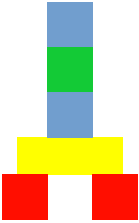
\includegraphics[scale=0.20]{figures/chapter2/task_goal.pdf}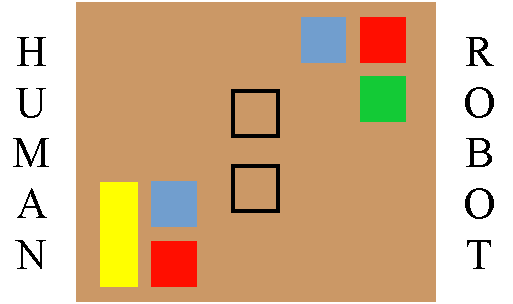
\includegraphics[scale=0.18]{figures/chapter2/task_setup_mini.pdf}}   
	\fancyhead[RO]{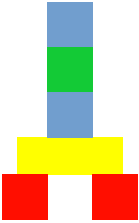
\includegraphics[scale=0.20]{figures/chapter2/task_goal.pdf}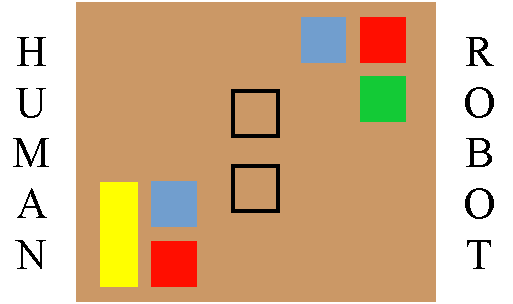
\includegraphics[scale=0.18]{figures/chapter2/task_setup_mini.pdf}\bfseries\thepage}  
	\fancyhead[RE]{\bfseries\nouppercase{\leftmark}}      % Chapter in the right on even pages
	\fancyhead[LO]{\bfseries\nouppercase{\rightmark}}     % Section in the left on odd pages
}%

\usepackage{pdfpages}
\usepackage{makecell}
\usepackage{pdflscape} 
\usepackage{mathtools}
\usepackage[section]{placeins}
\usepackage{afterpage}

%%%%%%%% my commands
\newcommand{\etal}{\textit{et al}.}
\newcommand{\ie}{\textit{i.e.}, }
\newcommand{\eg}{\textit{e.g.}, }
\newcommand{\fact}[3]{\mbox{\textit{#1}(#2, #3)}}
\newcommand{\circledtext}[1]{\raisebox{.5pt}{\textcircled{\raisebox{-.9pt} {#1}}}}
\newcommand{\sparql}{\textsc{SPARQL}}

\newcommand{\algConst}[1]{${\scriptscriptstyle #1}$}
\newcommand{\algNormTextSub}[2]{$\text{#1}_{#2}$}

\newcommand{\aslnumber}[1]{$#1$}
\newcommand{\aslstring}[1]{\textsf{#1}}
\newcommand{\aslvar}[1]{\textcolor{purple}{\textit{#1}}}
\newcommand{\asllabel}[1]{\textbf{#1}}
\newcommand{\annotation}[1]{{\footnotesize #1}}
\newcommand{\rulebody}[1]{\mbox{\hspace{.05\linewidth}}\begin{minipage}[t]{0.9\linewidth}#1.\end{minipage}}
\newcommand{\context}[1]{\begin{minipage}[t]{0.9\linewidth}#1\end{minipage}}
\newcommand{\planbody}[1]{\begin{minipage}[t]{0.9\linewidth}#1.\end{minipage}}
\newcommand{\Jason}[0]{\textbf{\textit{Jason}}}
\newcommand{\sn}{\mbox{\large\textbf{\texttt{\textasciitilde}}}}


\sloppy
\begin{document}
\setcounter{chapter}{4} %% Numéro du chapitre précédent ;)
\dominitoc
\faketableofcontents
\fi

\chapter{The Director Task: a Psychology-Inspired Task to Assess Cognitive and Interactive Robot Architectures}
\chaptermark{The director task}
\label{chapter:chap4}
\minitoc

In this chapter, we propose a new psychology-inspired task, gathering perspective-taking, planning, knowledge representation with theory of mind, manipulation, and communication. Along with a precise description of the task allowing its replication, we present a cognitive robot architecture able to perform it in its nominal cases. In addition, we suggest some challenges and evaluations for the Human-Robot Interaction research community, all derived from this easy-to-replicate task.

The contribution presented in this chapter is excerpted from our work, published in the proceedings of the RO-MAN 2021 conference~\cite{sarthou_2021_director}. This contribution has been achieved in collaboration with other PhD students of the \acrshort{hri} teams, our mutual thinking leading to the formulation of this new task for \acrshort{hri}. Then, more specifically in relation to the software implementation, Guilhem Buisan was concerned about the task planning part. Guillaume Sarthou worked on the knowledge management. Kathleen Belhassein has designed the presented task with us giving her psychologist point of view to create a task on which user studies could be performed. The engineer Yannick Riou worked on the motion planning component allowing us to develop a task where the robot acts on its environment. My involvement in this task was on the supervision component. It was an evolved version of the one which ran for the direction-giving task presented in the previous chapter, \ie the \acrshort{jahrvis} as described in Chapter~\ref{chapter:chap2}. It has also been the opportunity to refine the architecture developed for the \acrshort{mummer} project, leading to the one presented in this paper.


\section{Introduction}

Developing robotic architectures adapted to Human-Robot Interaction and thus able to carry out interactions in an acceptable way is still today a real challenge. The complexity comes, among other things, from the number of capabilities that the robot must be endowed with and therefore from the number of software components which must be integrated in a consistent manner. Such architectures should provide the robot with the capability to perceive its environment and its partners, to merge and interpret this perceptual information, to communicate about it, to plan tasks with its partner, to estimate the others' perspective and mental state, etc. Once developed, the evaluation of these architectures can be difficult because all these components grouped into a single system. The tasks we usually want the robot to handle must highlight a maximum of abilities, while still being simple enough to be reproduced by the community. Moreover, we should be able to conduct user studies with it to validate choices regarding naive users.

Since a long term goal of the robotic field is to see robots evolving in our daily life, many tasks and scenarios have been inspired by everyday activities. Even if these tasks offer a large variety of situation to be handle, since the human partner is not limited in his actions, they have the disadvantage of not highlighting some subtle abilities which are nevertheless necessary for good interaction.
The robot guide task \cite{satake_2015_should} in mall, museum, or airport, requires high communication skills to understand free queries (possibly involving chatting) and respond to them, whether to indicate a direction or to give advice. However, the perception needs can be limited due to the vast environments, as well as the perspective-taking needs due to the same perception of the environment by the robot and the human\footnote{For sure we can find some tricky cases where it could help but they do not reflect common situations.}. Finally, with such a task the human partner is not an actor of the task and just has to listen to the robot once their question is asked. Even if being in more constrained environments, bartender-like tasks~\cite{petrick_2012_social} have the same disadvantages. Indeed, the human is considered as a customer, and as such, the interaction with the robot is limited. The robot will never ask the human to help it for performing a task and their actions do not require coordination either full collaboration.

To involve the human partner in the task and requiring him to act with the robot, assembly-like tasks~\cite{tellex_2014_asking} can be used. Nevertheless, in most cases, the human acts as an assistant rather than as a partner as full collaboration can be challenging to perform. The robot thus elaborates a plan and performs the assemble, then asks for help when detecting errors during the execution (\eg when it cannot reach some pieces). Here the task leads to unidirectional communication. Moreover, because in such a task both the robot and the human have equivalent knowledge about the environment, it can be hard to design situations where belief divergence appears and thus perspective-taking would be required.

Scaling down an everyday task to transform it into a toy task around a table can reduce the task complexity and allow easy reproducibility. Moreover, it allows the robot and the human to work in the vicinity of each other, with smaller robots for example. With the toy version of the assembly task presented in~\cite{brawer_2018_situated}, the human is more involved in the task. They ask the robot to take pieces and to hold them to help them assemble a chair. Even if the communication is unidirectional, we could imagine inverting the roles to test different abilities. Moreover, communication implies objects referring with the use of various visual features about the entities. Even if both agents have the same knowledge about the environment, the communication is grounded according to the current state of the world. In this task, no decision has to be made by the robot but once again, inverting the roles could open other challenges.

To focus studies around perspective-taking and belief management, the Sally and Anne scenario, coming from a psychology test, has been studied in robotic~\cite{milliez_2014_framework}. In this scenario, the robot is an observer of a situation where two humans come and go from a room, and move an object from a box to another. Since a human is in the room when the other is acting, a belief divergence appears between the two humans and the robot has to understand it. While the task highlights the belief management, it is first limited regarding the perspective-taking since the human presence or not could be sufficient to estimate the humans beliefs\footnote{When both humans are in the room they have the same perception of the scene but have different beliefs about hidden objects. Perspective-taking would be required if the humans could lean over the boxes to check what is inside.}. Moreover, the humans do not act with the robot since it is just an observer of the scene. In addition, no goal is formulated and the human neither interacts with one another. Finally, no communication is needed in the task. The scenario is thus focussed on the analysis of a situation.

In this chapter, we first propose a new psychology-inspired task that we think to be challenging for the Human-Robot Interaction community and rich enough to be extended: the Director Task. Inter alia, it requires perspective-taking, planning, knowledge representation with theory of mind, manipulation, communication, and decision-making. Then, we present the robotic cognitive architecture that we develop to perform the task in its nominal cases. Finally, on the basis of the presented task and what has been developed, we present a discussion about the possible future challenges and evaluations for the research community, with possible extensions of the task.

\section{The Director Task: From psychology to Human-Robot Interaction}

In this section, we present the origins of the Director Task and the needs it aims to respond to regarding other tasks from the psychology. Then, we detail the setup we have designed in terms of objects characteristics and organization in the environment. We end this section with our adaptation and the required abilities we have identified.

\subsection{The original task}\label{chap4:subsec:psycho}

The Director Task has been mainly used in psychology as a test of the \acrfull{tom} usage in referential communication. This task originates from a referential communication game from Krauss and Glucksberg~\cite{krauss_1977_social}. In this game, two participants are one in front of the other with an opaque panel between them. A speaker has to describe odd designs to a listener, either to number them for the adults or create a stack of cubes for the children. To refer to the odd figures, participants have to use images (\eg ``it looks like a plane'').

This game was then adapted by Keysar \etal~\cite{keysar_2000_taking} and became the Director Task. It has been used to study the influence of mutual knowledge in language comprehension. In this task, two people are placed one in front of the other but instead of an opaque panel between them, they place a vertical grid composed of different cells and objects in some of them. The \textbf{director}, a participant or in most cases an accomplice, instructs the \textbf{receiver}, a participant, about objects to move in the grid. The receiver thus follows the director's instructions about objects to move. The particularity of the task is that some cells are hidden from the director, meaning that the receiver, being on the other side of this grid, does not have the same perspective as the director. They thus know the content of more cells than the director and consequently sees more objects. When the director instructs the receiver to move an object, for a successful performance, participants must take the perspective of the director to move the right one. Because the configuration evolves all along with the task, they have to update their estimated perspective all along with the interaction.

\begin{figure}[ht!]
	\centering
	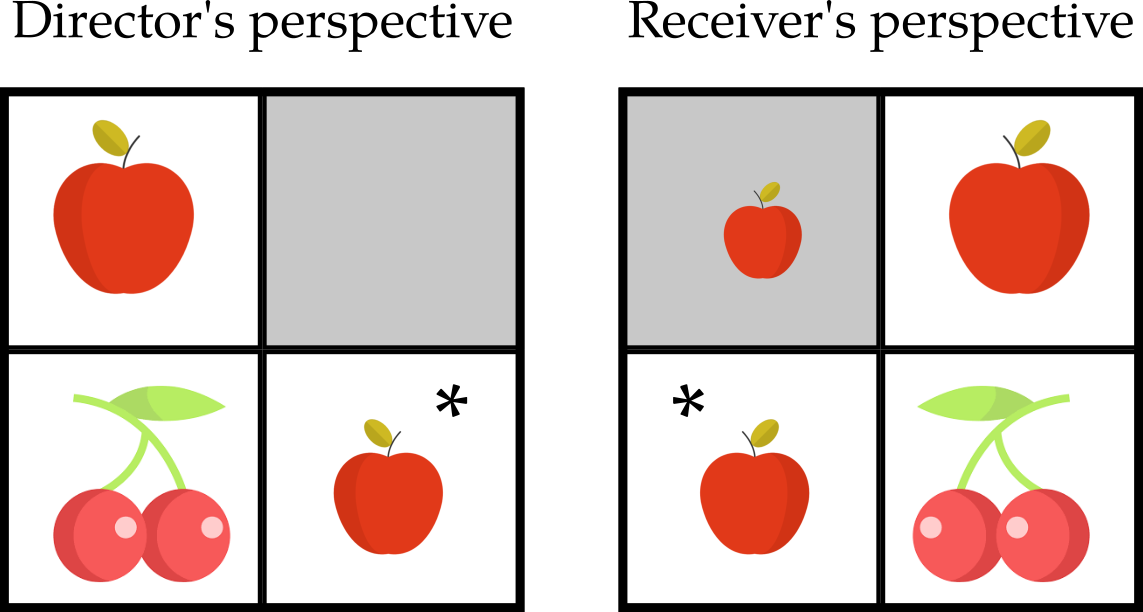
\includegraphics[scale=0.25]{figures/chapter4/dt_apple.png}
	\caption{\label{chap4:fig:dt_apple} Sample display from the director's and the receiver's perspectives. The asterisk indicates the target object. Giving the sentence ``the smallest apple'' the receiver should find the good one even if he can see a smallest one in its perspective. }
\end{figure}

For example in Figure~\ref{chap4:fig:dt_apple}, if the director asks for the smallest apple (*), the proper smallest (called competitor) is only visible by the participant and not by the director. The participant then must understand the director's perspective to take the target apple and not the competitor one. Some studies showed that for their first attempt, participants considered or took the smallest apple from their own point of view and only after, the target one. These results were interpreted in various works as the participants understanding language in an egocentric way~\cite{keysar_1994_illusory, keysar_1998_egocentric, keysar_2002_self, keysar_2003_limits}. 
Some social cognition studies used a computer-version of the Director Task whose results are consistent with the ones mentioned previously, namely that participants do not use \acrshort{tom} inferences in language interpretation~\cite{dumontheil_2010_online}.

Although they require the attribution of mental states to others, some authors have distinguished \acrshort{tom} tasks and perspective-taking tasks reporting distinct although related mechanisms. Santiesteban \etal{}~\cite{santiesteban_2012_training} considered in their study that perspective-taking abilities were measured by the Director Task whereas \acrshort{tom} usage was investigated through another task called ``strange stories''~\cite{happe_1994_advanced}. However, this \acrshort{tom} task requires the attribution of mental states to a story protagonist (to have knowledge of others' mental states), whereas the Director Task asks for adopting the perspective of the director in order to follow their instructions (to use this knowledge in order to execute the task properly). Thus, the authors estimated that the Director Task requires a higher degree of self-other distinction by continuously isolating our own perspective from the director one. In addition to perspective-taking abilities, the Director Task makes use of executive functions~\cite{rubio_2017_director} and attentional resources~\cite{lin_2010_reflexively}.

The Director Task has thus been particularly used in psychology studies of referential communication, language comprehension, and perspective-taking abilities. However, to date it has never been exploited in the context of a HRI although this task presents interesting challenges for this field. It would not only bring technical challenges but also provide a way to investigate the different cognitive and behavioral processes involved in such a cooperative Human-Robot task.

\subsection{The Director Task setup}\label{chap4:subsec:material}

The material used in this task has been chosen to be easily acquired and can be hand-built. It is composed of blocks, compartments, and a storage area. Each element is equipped with AR-tags allowing the robot to perceive them without advanced perception algorithms.

\begin{figure}[ht!]
	\centering
	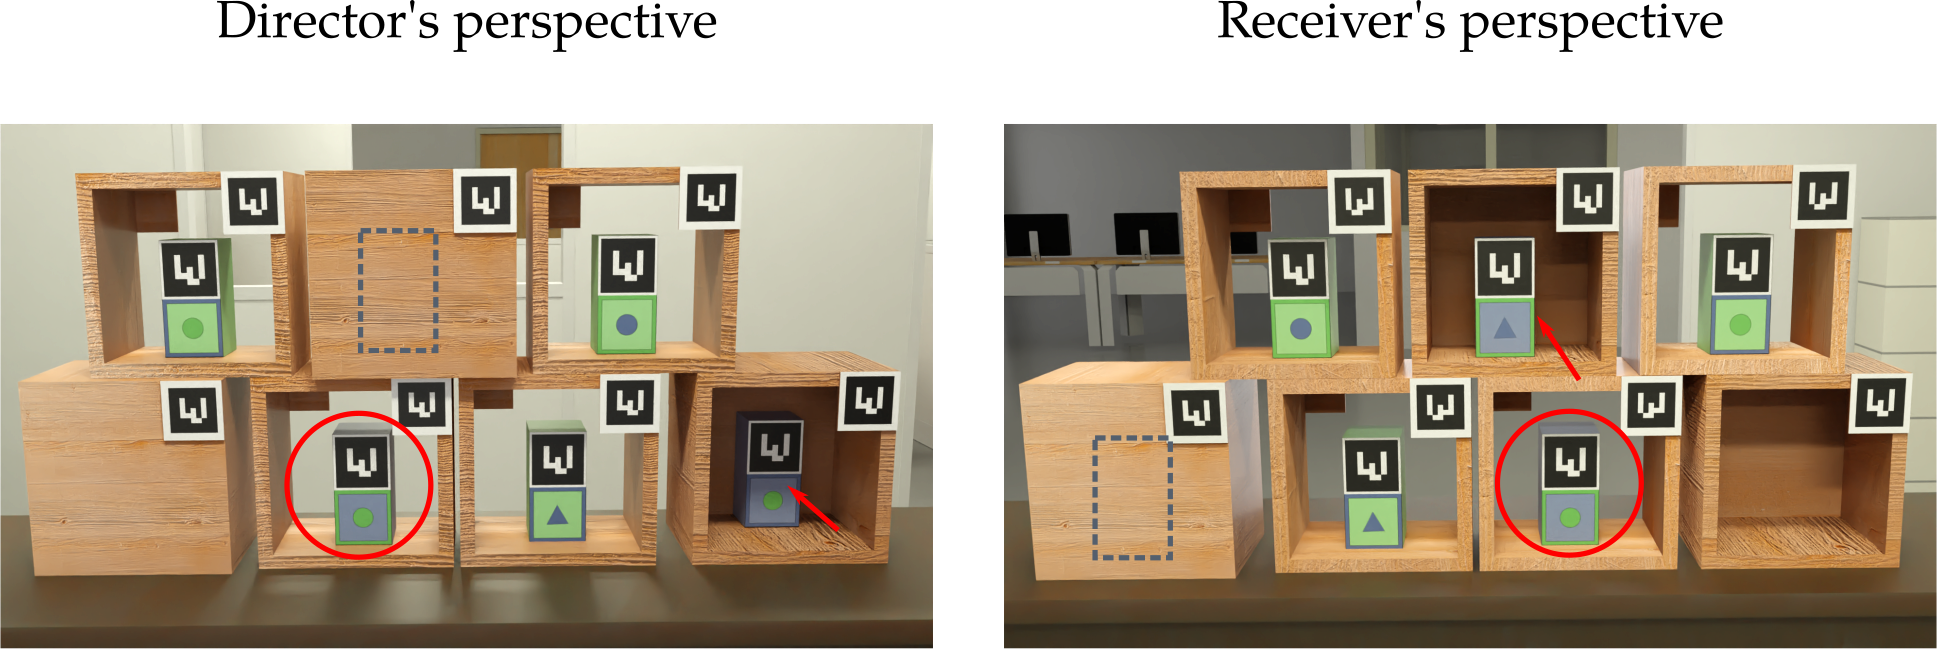
\includegraphics[width=\textwidth]{figures/chapter4/setup.png}
	\caption{\label{chap4:fig:setup} A director task setup adapted to the \acrshort{hri} with the director's and receiver's perspectives. For the material, each element (blocks and compartment) is equipped with AR-tags allowing their detection by the robot. Each block has four visual characteristics: a main color, a border color, a geometric figure, and a figure color. Compartments can be hidden for the director or the receiver. For the director to designate the block marked with a red circle, estimating the receiver's perspective, he can refer to it by its main color (blue) because he estimates the other blue block is not visible by the receiver. For the receiver, by taking into account the director's perspective, he can understand the referred block as he estimates the other blue block to not be visible by the director.}
\end{figure}

As shown in Figure~\ref{chap4:fig:setup}, the blocks have a primary color covering them all. On two opposite faces, additional visual features are drawn. The top part of these faces is dedicated to the robot's perception with unique AR-tag on each face\footnote{because the tags are different on each side, the director can not refer to them as the receiver does not see the same ones}. The bottom part is the same on both faces and is dedicated to the human perception with a main color, a border, and a geometric figure. Every visual feature (the colors and the forms) has exactly two variants. The colors are either blue or green and the figures are either a triangle or a circle.
The figures and colors have been chosen in such a way to allow the emergence of ``coded words'' between the participant to identify a block. With a bit of imagination, some could refer to the left-most block through the sentence ``the mountain in the sea'' or the second leftmost by ``the puddle''.
The number of features has been chosen to have sixteen block variants from which we remove the four uni-color variants (all the elements having the same color) to avoid too easy description of the kind ``the fully green block''.
Regarding their description complexity, while the main color is directly related to a block, the other colors are respectively related to the border and the figure. This means that for two blocks whose only difference is the color of one of these elements, the said element has to be referred to by its color. A description of a block involving all its features would be ``the [color] block with the [color] border and the [color] [figure]''. Such complete descriptions are hard for the human to process. In this way we expect the participants to minimize the complexity of their communication by referring to the blocks only using the features distinguishing them from other blocks.

Three types of compartment exist. Some are open on two of their opposite sides allowing both the receiver and director to see the content and to manipulate it. Some are open only on one of their sides meaning that only one of the participants can see and take what is inside. The other participant can thus neither know if a block is inside or not. The last compartment type has an open side and the opposite one equipped with a wire mesh. Because of the side with the wire mesh, both participants can see what is inside but only one of them can take it. With these three types, we will be able to test the impact of the awareness of the blocks (\eg a block is known to be present but not necessarily visible), the visibility of the blocks, and their reachability (\eg a block can be visible but not reachable).

Finally, one storage area, corresponding to the place where the receiver has to store the blocks, is delimited by a rectangle on a shelf.

\begin{figure}[ht!]
	\centering
	\includegraphics[scale=0.15]{figures/chapter4/positions.png}
	\caption{\label{chap4:fig:positions} The Director Task setup with the robot and the human partner one in front of the other and a piece of furniture between them. Compartments are placed on top of the furniture and blocks are placed in the compartments. Next to the agent having the receiver role, here the human, a storage area is placed to drop the removed blocks. }
\end{figure}

Regarding the disposition, the compartments are stacked on a piece of furniture to create a kind of grid. The blocks can be put in a compartment. As illustrated in Figure~\ref{chap4:fig:positions}, the two agents are placed one in front of the other with the furniture and thus the compartments between them. Finally, one storage area, corresponding to the place where the receiver has to store the blocks, is delimited by a rectangle on a shelf next to the receiver. In the figure, the human would be the receiver since he has the storage area on his right.

\subsection{The Director Task adaptation for HRI}

In this section, we present the DT-HRI, the Director Task as we designed it for HRI, keeping the principle of two participants with a vertical grid between them. The high-level goal of the task is known by both agents: to put a set of blocks away. The precise goal is given by the experimenter to the director, either the robot or the human, i.e., the set of blocks that the receiver should remove from the compartments (see Figure~\ref{chap4:fig:setup}).

As mentioned in the previous section, the Director Task characteristics bring a number of interesting  challenges for a collaborative robot to solve. Because this is a task with two roles, one of the first challenges is to build a robotic architecture that gives the robot the ability to play both roles. Then, each role brings some problems to solve from a robotic point of view. 

In the original task, the director knows they have a subset of the receiver's perspective, they can consider all the objects when communicating. Thus, only the receiver has to reason about the other's perspective, taking into account that some objects are not visible by the director. In order to enrich the task for HRI application, we propose to also have compartments hidden from the receiver and visible by the director (see Figure~\ref{chap4:fig:setup}). Therefore, both roles have to perform perspective-taking, whether to give instructions or to understand them.
On one hand, this challenging task allows to demonstrate the abilities of a robotic system. On the other hand, it is an easily reproducible scenario to perform user studies on human-robot interactions in a controlled environment. 

To be able to study more specifically some skills, such as verbal communication, perspective-taking and adaptation, we defined a set of rules for both the robot and the participant. First, to focus the task on verbal communication, the agents are \textbf{not allowed to point} to objects, either with their hand or gaze. Then, to strengthen the perspective-taking aspect and not fall into a simple referential communication task, participants are \textbf{not allowed to use geometrical relations} in the verbal communications. They cannot, for example, say ``the leftmost block'' or ``the block to the right of the green one''. In this way they are limited to few visual features, with high ambiguity, therefore requiring to take into account the other perspective. Finally, to enable an evolution of the situation over time and thus requiring a constant adaptation during the interaction, the objects are not moved from one compartment to another but removed from the compartments. The \textbf{order of the instructions is free}, enabling the director to elaborate a strategy if needed.

\subsection{A task to demonstrate the abilities of a robotic system}\label{subsec:abilities}

More than being an easily reproducible scenario to perform user studies on human-robot interactions in a controlled environment, the Director Task allows to demonstrate abilities of a robotic system. We detail here some abilities for which the task has been designed for.

paragraph{Perspective-taking abilities} When working on the ToM in the HRI context, the Sally-Anne test has been used multiple times and allowed to demonstrate some systems~\cite{milliez_2014_framework}. But, one of the benefits of the Director Task compared to the Sally-Anne test is that the agents (human or robot/director and receiver) have not only to infer knowledge using the other's point of view but also to act so it is possible to acknowledge that they use it in decision-making. 

\paragraph{Communication abilities} Moreover, the task 
requires to put a focus on communications which is widely studied in HRI. Indeed, the communication about an object can be more or less efficient, depending on the number of characteristics given about the object or the pertinence of these characteristics (\eg in Figure~\ref{chap4:fig:dt_apple}, the director does not need to add ``red'' to ``take the small apple'' as there is no apple of a different color). The robot needs to be able to give proper instructions but also to understand the human ones.

\paragraph{Planning abilities} When a large number of blocks has to be taken in the task goal, it quickly becomes complicated to communicate about some of them as the director would have to add a lot of adjectives to be able to refer to one block. Therefore when the robot is the director, it becomes interesting to integrate the communication and the task planning together. Indeed, depending on the order in which the blocks are designated, the complexity of instructions can decrease or increase. Then, the planner can return an optimal order in which the robot has to give the instructions to the human.

\paragraph{Contingencies handling abilities} While performing the Director Task, errors can happen. Either because the director gives a wrong instruction or the receiver misunderstands the instruction and takes the wrong block. In both cases, it can be because of a wrong consideration of the other agent's perspective. In the latter case, the instruction might be right but hard to interpret by the receiver leading to an error from them. Finally, errors can happen because of a failed action execution (\eg a block falls on the floor), a system failure for the robot, inattention from the human, etc. A robot with a robust decision-making system will be able to analyze, try to determine their origin, and handle a number of these contingencies. For example, if the human takes the wrong block, the robot can react in different ways, \eg asking the human to put it back or saying nothing and re-planning if this block was among the ones to take. If errors happen repeatedly, the robot can react differently than for a punctual error.


\section{The cognitive robot architecture}
\label{chap4:sec:archi}

In this section, we present the architecture developed to handle the Director Task in its nominal case but also to allow for future extensions, endowing the robot with the abilities described in section~\ref{subsec:abilities}. The architecture is basically the one presented in Section~\ref{chap2:sec:rob_archi}.
The seven identified modules are represented in Figure~\ref{chap4:fig:architecture} with their respective communication links. In the rest of the section, we detail each module and how we have refined them in terms of functionality and linking.

\subsection{Storing and reasoning on symbolic statements}

As seen in the previous chapters, knowledge allows the robot to understand the environment it evolves in. Moreover, this same knowledge makes the robot able to communicate with its human partner about the current state of the world and ground the partner's utterance regarding this same world state.

Some have chosen to propagate their knowledge all along their architecture~\cite{hawes_2007_balt}, each component enriching this knowledge at each stage. Others have preferred to see their knowledge base as an active server activating perception process regarding the searched information when needed~\cite{beetz_2018_know}.

As the architecture on which we based ours, we chose a central, server-based, knowledge base. We however refined it into two distinct sub-modules, the semantic knowledge base and the episodic one, as presented in Chapter~\ref{chapter:chap2}, managed by Ontologenius.

\begin{figure}[t!]
	\centering
	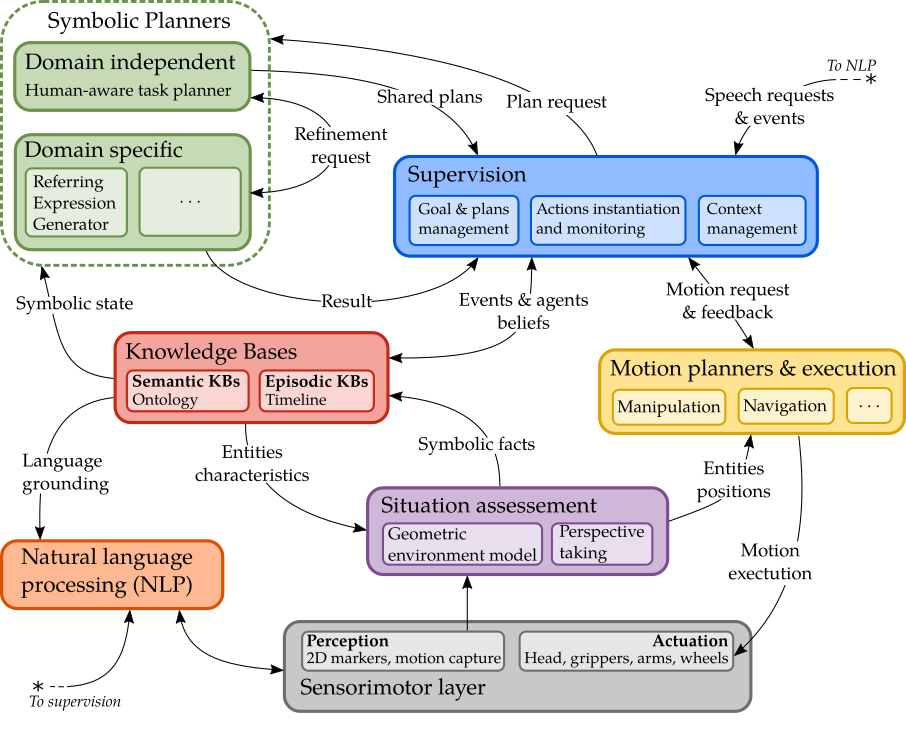
\includegraphics[scale=0.40]{figures/chapter4/architecture.png}
	\caption{\label{chap4:fig:architecture} An overview of the architecture developed to handle the Director Task. Each block does not necessarily represent one software component but rather an architectural module (in terms of the features it implements). The arrows represent the type of information exchanged between the modules.}
\end{figure}


\subsection{Assessing the world: from geometry to symbolism}

The role of the geometrical Situation Assessment module is first to gather different perceptual information and build an internal geometric representation of the world. From this world representation, the module then runs reasoners to interpret it in terms of symbolic statements between the objects themselves and between the involved agents and the objects. Doing so, the module only builds the robot's representation that does not necessarily reflect what the human partner believes about the world. This is the case with the occluded compartments. If a block is present in a compartment occluded from the human perspective, this block is not visible and thus unknown to the human and should not exist in their representation of the world. Here is the second role of our Situation Assessment module, estimating the human's perspective and building an estimation of their world representation. It is the first step allowing to implement the \acrshort{tom} principles (see Section~\ref{chap1:subsec:tom}).

To implement this module, we have chosen the Underworld framework~\cite{lemaignan_2018_underworlds}. It has the advantage to not be monolithic. Its principle is to create a set of worlds, each working at a different granularity and integrating specific features. It allows easy reuse of existing modules and makes the core reasoning capabilities independent of the used perception modalities. The worlds' structure we use is represented in Figure~\ref{chap4:fig:uwds}. At the top, there are the perception modalities, here AR-tags~\cite{fiala_2005_artag} for the objects and motion capture (mocap) system for the human detection. For each perception system, we define a world. In these worlds, we can filter the perception data depending on the system used. For the mocap, the data is clean enough. For the AR-tags we apply first a motion filter to discard data acquired when the robot moves and a field of view (FOV) filter to discard data from the border of the camera because of distortions. Moreover, both perception worlds can use the knowledge base presented previously to get the entities' CAD models and unique identifiers (UIDs) shared across all the components of the architecture. When the AR-tags world receives an AR id, it can query the semantic knowledge base to get the UID related to this tag and get its CAD model. As the output of these worlds, we ensure to have clean data with UID related to the knowledge base.

\begin{figure}[b!]
	\centering
	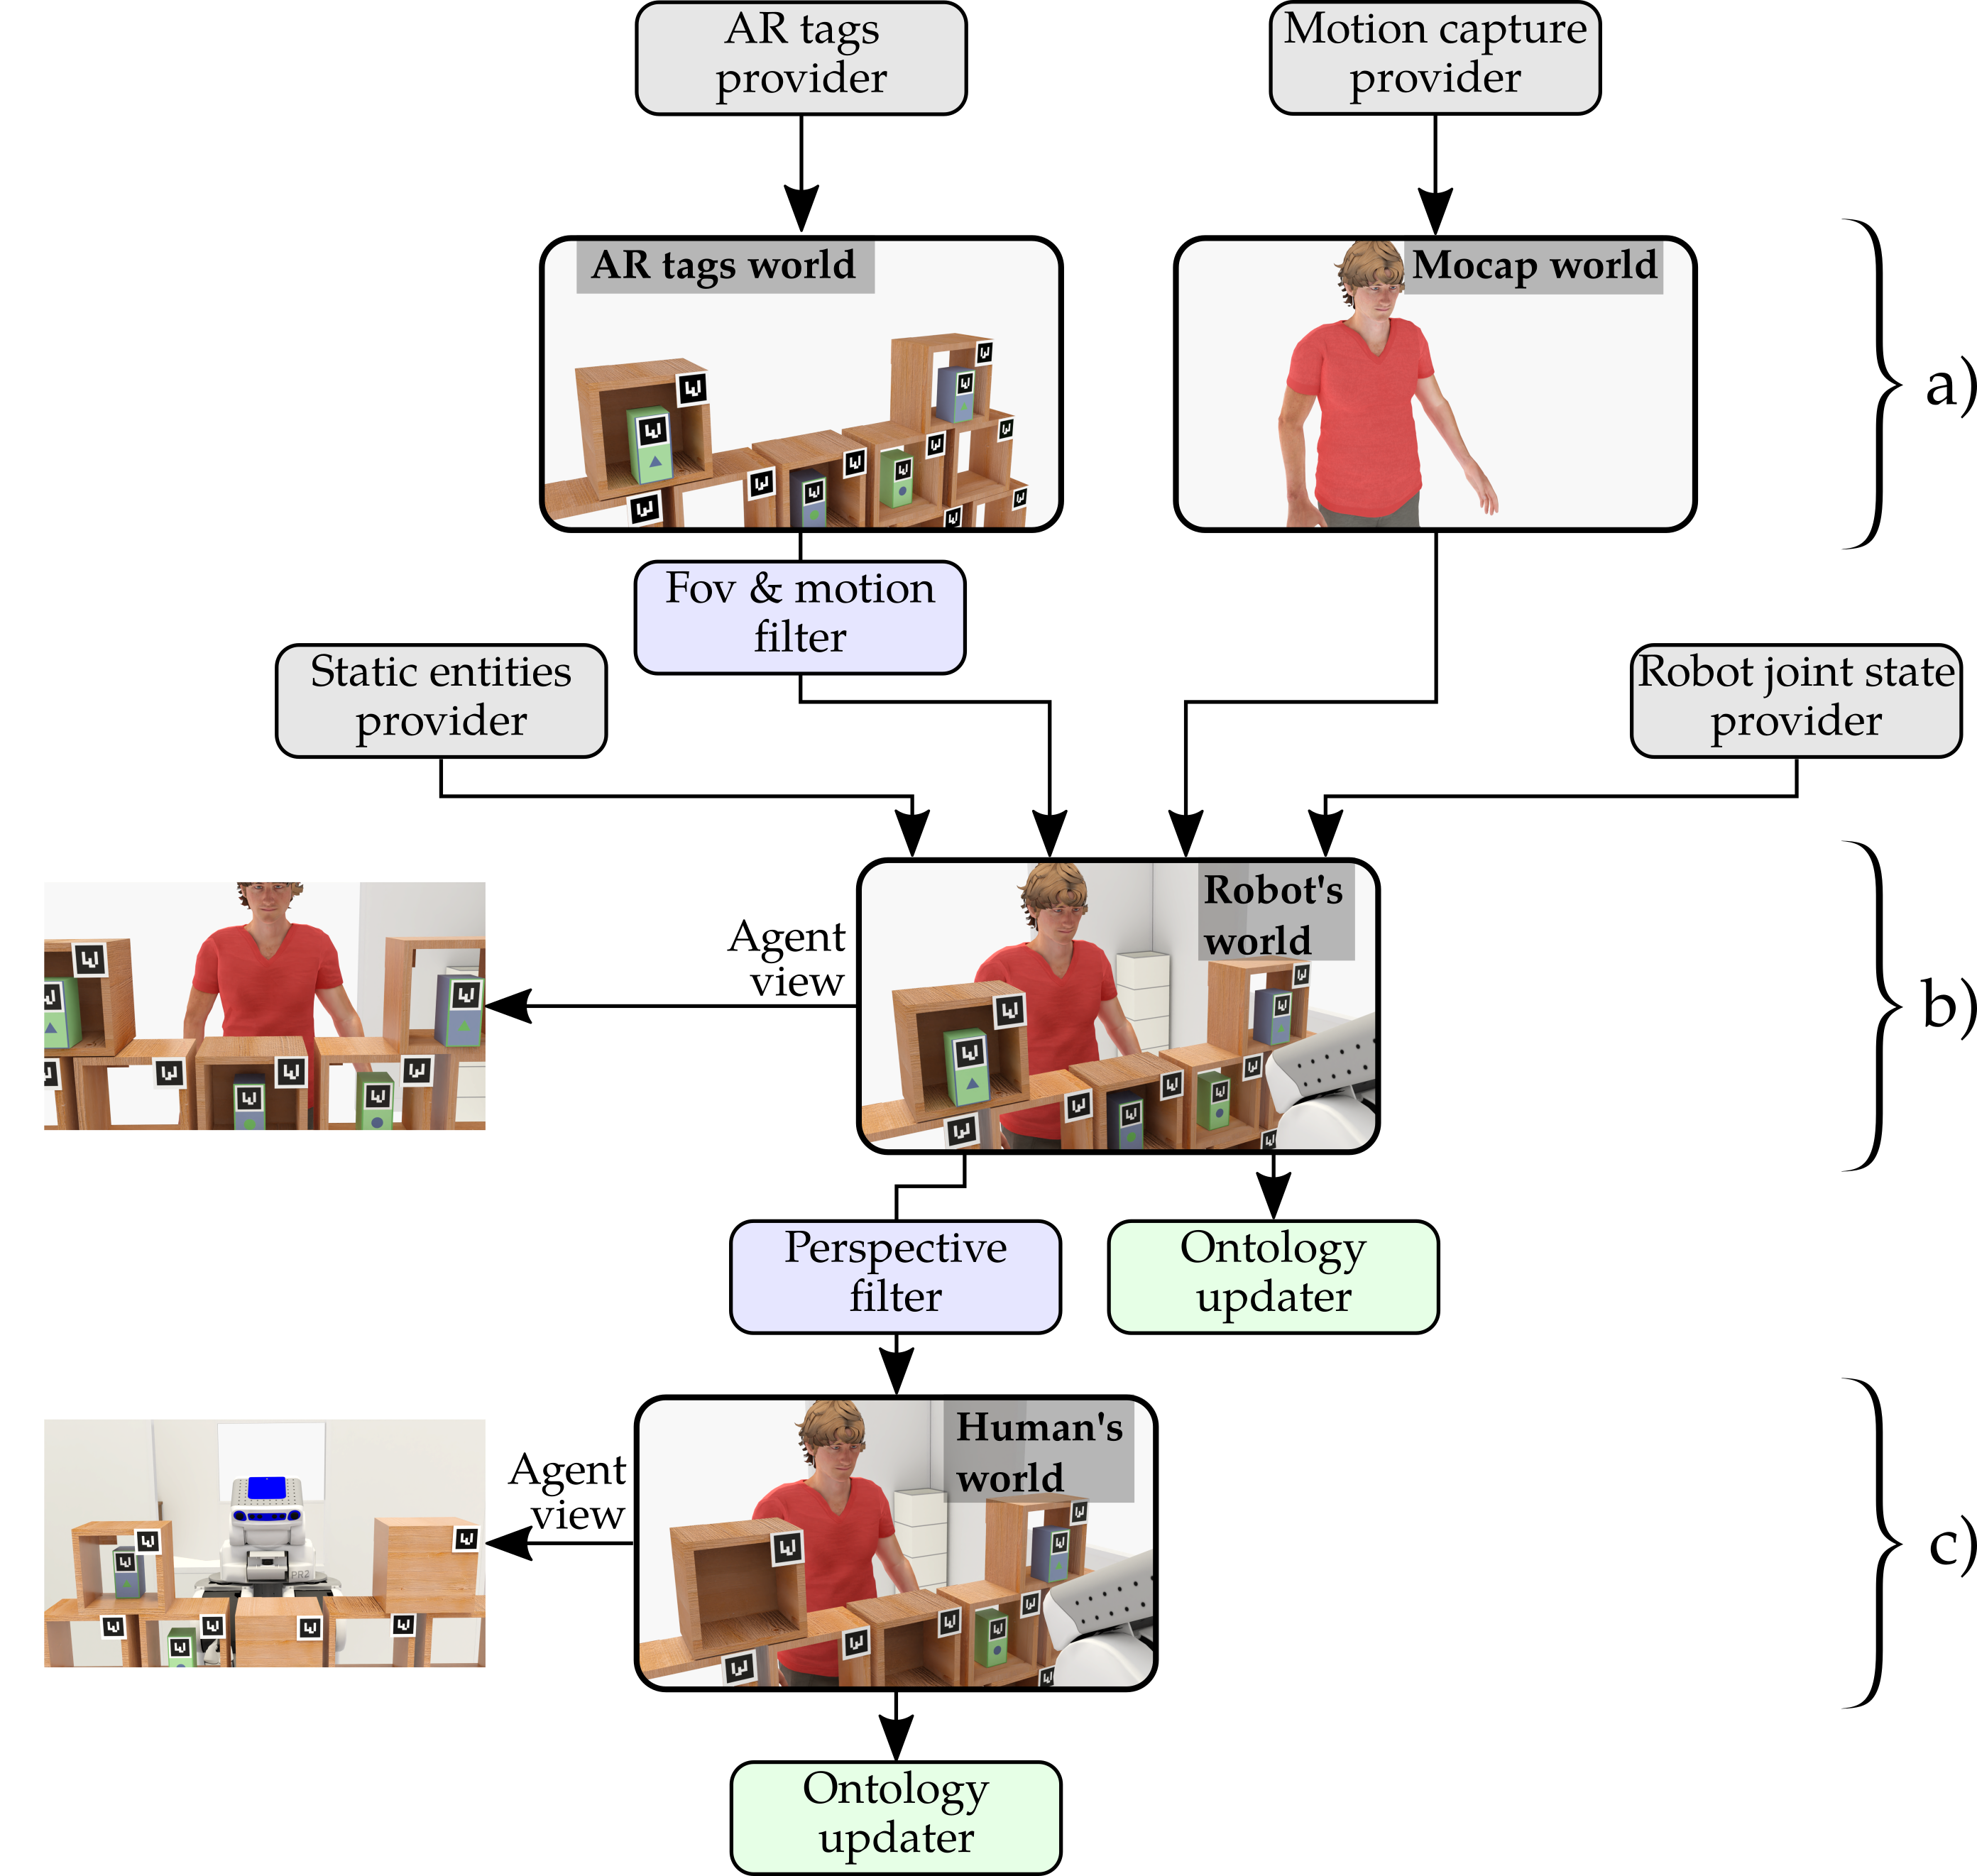
\includegraphics[scale=0.12]{figures/chapter4/uwds/uwds.png}
	\caption{\label{chap4:fig:uwds} The world cascading structure of the geometrical situation assessment system. The two worlds at the top are build from the perception systems and filtered. The world of the middle merges the different perception information and computes symbolic facts on it. The world at the bottom is the estimation of the human world representation and is computed based on perspective-taking in the robot's world. Like for the world of the middle, symbolic facts are computed and sent to the semantic knowledge base.}
\end{figure}


The world of the middle in Figure~\ref{chap4:fig:uwds} is the robot's world representation. Information from the perception worlds is merged along with the static elements (the building walls) and the robot model.
%From this world, additional perception reasoning processes are applied for the objects that are no more visible in the way of~\cite{milliez_2014_framework}. If an entity is no more perceived in one of the previous worlds, the algorithm first tests if it should be in the robot's FOV. If so, the robot should see it. It thus tests if another entity could hide it. If not, the object is removed from the world representation and kept otherwise. 
From there, geometric reasoners are applied to extract symbolic facts. In the current version of the system, the computed facts are \textit{isOnTopOf}, for an object put on top of another, \textit{isInside}, for a block in a compartment, \textit{isVisibleBy}, assessing if an agent could see the object or not, and \textit{isReachableBy}, assessing if an object can be taken by an agent. All these facts are sent to the robot's semantic knowledge base, where reasoners will deduce further facts. For example, if a block is in a compartment, the compartment has the block inside (inverse property), and if this compartment is on top of the table, the block inside is also above the table (chain axiom).

While the previous world corresponds to the robot's representation, the one below aims at representing the partner's one. From the previous world, we compute a segmentation image from the human point of view and use it as a filtered perception world. This allows us to instantiate the same kind of world management process we used for the robot but this time for the human. In this way, we emulate their perception capability and the geometric reasoners can be run in the same way as previously. Symbolic facts are thus computed and sent to the human's semantic knowledge base. In the world of the bottom on Figure~\ref{chap4:fig:uwds}, we can see that the two blocks in the occluded compartments are not present in the human world. Here we make explicit the difference between an object that is unknown and an object that is known but not visible.


\subsection{Planning with symbolic facts}

The symbolic planners are divided into two categories: the domain-independent, planning high-level tasks, and the domain-dependant, specialized in solving precise problems. We first introduce the domain-specific ones and the domain-independent in a second time.% as it takes advantage of the previous ones.

\subsubsection{Solving precise problems}

Building a single monolithic planner could be an intractable challenge. Thus, we chose to consider a set of dedicated planners which could be reused from one system to another. In the current version of the system, only one specific planner has been identified. This planner is a \acrfull{reg} solver. Regarding the current symbolic state of the world, it aims at finding the minimal set of relations to communicate and allow the listener to identify a given entity. For example, wanting to refer to a block being the only one with a green triangle on it among the other, this planner can find that the only relations to communicate are the block's figure and the figure's color. With this information, the listener should be able to identify the referred block without ambiguity.

This planner is presented in~\cite{buisan_2020_efficient} which is based on a Uniform Cost Search algorithm and which is to the date the most efficient one in term of computation time. It works with an ontology, being the semantic knowledge base presented previously. Because the communication information it generates will be interpreted by the robot's partner, we chose to give the estimated human knowledge base as input to the planner. Thanks to this, the blocks unknown from the human --- i.e., hidden from them --- are not taken into account as they cannot lead to any ambiguity for the listener. Moreover, this planner can take some constraints as input, related to the property usability and the context of the communication. The usable properties constraint prevents some properties to be used in a referring expression. Indeed, the input ontology is not dedicated to the specific referring expression generation problem and contains additional knowledge used by other modules as the objects' CAD models or tag UIDs, that does not aim to be communicated. The communication context aims at representing relations assumed to be already known by the listener. For the Director Task, when the robot asks the human to take a block, it assumes they know it is only talking about objects above the table around which the robot and the human are interacting. The already stored blocks --- not on the table anymore --- are thus not taken into account in the communication. If needed the communication context can be refined, for example by defining that the robot --- and thus should the human as well --- will only consider visible blocks and reachable blocks.

\subsubsection{Planning for self and others}

In the context of a Human-Robot interaction, when planning how to perform a high-level task, one has to take into account the human's contribution. Our current task planner is \acrshort{hatpehda} mentioned in Section~\ref{chap2:subsec:plan_handling}. This planner allows the robot to plan by emulating the human decision, action, and reaction processes. For the Director Task, emulating the human reaction to a given instruction enables the comparison between multiple blocks order, the communication of higher-level instructions to the human (\eg ask to withdraw rather than take then put down) and the balance between multiple communication modalities.

As at execution time the supervision uses the \acrshort{reg}, a domain-specific planner, and because the task planner uses the same type of knowledge representation, thus \acrshort{hatpehda} can use this planner during its planning process. In the current architecture, it can thus estimate the cost and the feasibility of referring communication by calling the \acrshort{reg}.

\subsection{Managing the interaction}

Based on the components presented above, \acrshort{jahrvis} manages the execution of Director Tasks, based on its processes presented in Chapter~\ref{chapter:chap2}.


\section{Experiments}\todo{modifs pour axer supervision-texte de guillaume}

The architecture has been successfully implemented on a PR2 robotic platform. The robot is thus able to play both roles, the director and the receiver. In this section, we comment and analyze a video\footnote{\url{https://youtu.be/jtSyZeqBkp0}} of two experiments. For both experiments, the initial state is the same and are represented in Figure~\ref{chap4:fig:expe_config}. The only emulated element is the human action recognition to trigger the next actions of the robot when it holds the director role as at the time, the \acrfull{ham} process presented in Section~\ref{chap2:subsec:h_moni} was not developed yet.

\begin{figure}[ht!]
	\centering
	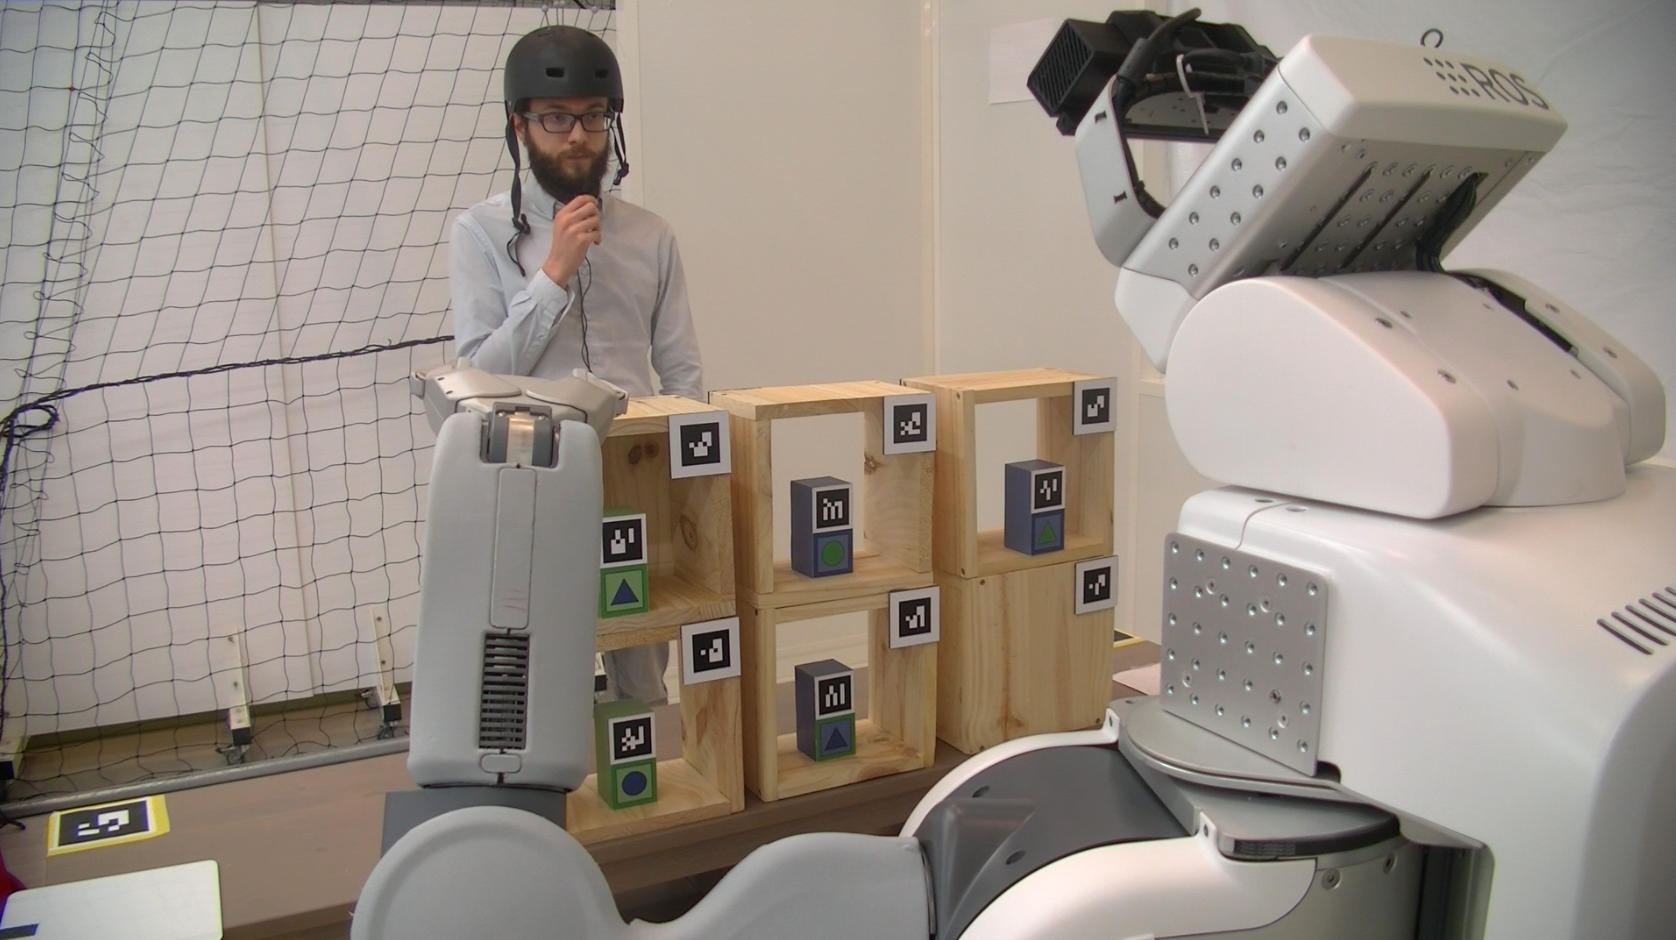
\includegraphics[width=\textwidth]{figures/chapter4/expe/config.png}
	\caption{\label{chap4:fig:expe_config} Initial configuration for both case studies. The top-right block is not visible, and thus unknown, by the human partner. The robot can not know if there is a block in the bottom-left compartment. All others blocks are known by both the robot and the human.}
\end{figure}

\subsection{PR2 as the director}

We start this section with a PR2 in the role of the director (0:21 in the video). The setup is composed of six compartments including two compartments with a hidden face. One of these compartments is hidden from the human (the receiver) and one from the robot (the director). One block has been placed in each compartment. Consequently, only four blocks are known by both the human and the robot. Figure~\ref{chap4:fig:robot_view} is a visualization of the estimated geometric world of the human, maintained by the situation assessment component. Even if a block is present in each compartment, the leftmost one is not present in the estimation of the human's world. This absence comes from the fact that the human can not see what is in the compartment and thus can not know this block.

\begin{figure}[ht!]
	\centering
	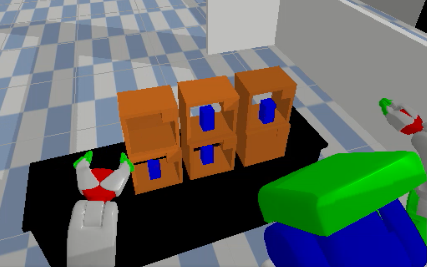
\includegraphics[scale=0.5]{figures/chapter4/robot_view.png}
	\caption{\label{chap4:fig:robot_view} A visualization of the human's estimated geometric world from a third-person view. Even if a block is present in each compartment, the right most one is not present in this worls since the human can not see this block. }
\end{figure}

Figure~\ref{chap4:fig:director} represents the entire interaction when the robot is the director. At the initial state, four blocks are visible from both agents. Describing them with all their visual features, they are:

\begin{itemize}
	\item A blue block with a blue border and a green triangle
	\item A blue block with a blue border and a green circle
	\item A blue block with a green border and a blue triangle
	\item A green block with a green border and a blue circle
\end{itemize}

Thanks to the estimation of the communication cost at task planning using the results of the \acrshort{reg}, the robot is able to find the optimal sequence of blocks to instruct. The overall communication is thus minimized and the RE is unambiguous in each situation. In the initial state (a to b), the robot asks for the green block as only one of the visible blocks is green. Since the green block has a circle on it, removing it, only one of the remaining blocks has a circle on it. The robot can thus use this feature to refer to the next block (b to c). Without communication cost estimation during the task planning, such a simple situation would not necessarily appear.

\begin{figure}[ht!]
	\centering
	\includegraphics[width=\textwidth]{figures/chapter4/director.png}
	\caption{\label{chap4:fig:director} The director task handled by an autonomous PR2 robot in the role of the director. Each picture represents a step toward the achievement of the task. The estimated human perspective is displayed in the top left-hand corner of each picture. On top of the arrows leading to a new state are the sentences said by the robot to the human. The block outlined in red are the blocks referred to at each step. }
\end{figure}

\subsection{PR2 as the receiver}

While in its previous role the robot just had to instruct the human, when the robot is the receiver (1:33 in the video) more reasoning is needed. A retranscription of part of the interaction is represented in Figure~\ref{chap4:fig:receiver}. In the initial state, the same four blocks as previously are visible by both the agents. The robot is able to understand three actions: take, drop, and remove. The latter action is a combination of the two others.

\begin{figure}[ht!]
	\centering
	\includegraphics[width=\textwidth]{figures/chapter4/receiver.png}
	\caption{\label{chap4:fig:receiver} The director task is handled by an autonomous PR2 robot in the role of the receiver. Each picture represents a step toward the achievement of the task. The estimated human perspective is displayed in the top left-hand corner of each picture. On top of the arrows leading to a new state are the sentences said by the human to the robot and for the last situation the refinement query from the robot to the human, followed by the answer of the human. }
\end{figure}

For the first block (a to b on the figure), the human instructs the robot for the green block. The natural language understanding module returns the \sparql{} query:

\begin{quote} 
	\centering 
	(?0, isA, Block), (?0, hasColor, green)
\end{quote}

Since the robot assumes the human to speak about objects on the table, the understood query is merged with another one representing the context of the task: (?0, isAbove, table\_1). Querying the human estimated ontology with the merged query, only one entity match. There is no ambiguity in human instruction. The robot takes the instructed block then drop it. If the query was applied to the robot ontology, two blocks would have matched since the block unknown by the human is also green. It goes the same for, the second instruction. There is no ambiguity. The \sparql{} query related to this second block is:

\begin{quote} 
	\centering 
	(?0, isA, Block), (?0, hasFigure, ?1), (?1, isA, Circle)
\end{quote}

The third instruction given by the human as the director is the most interesting for us. The human asks for \textit{``The block with a triangle''}. However, the speech to text returns \textit{``take is about to whip a triangle''}. With this sentence, the NLU module can only extract two known concepts being ``take'' and ``triangle''. Due to the limited amount of words understood, it does not try to generate a \sparql{} query. The robot thus informs the human about its incapacity and repeat the heard sentence as a back loop for the human. At the second try, the sentence is understood and gives the query:

\begin{quote} 
	\centering 
	(?0, isA, Block), (?0, hasFigure, ?1), (?1, isA, Triangle)
\end{quote}

However, matching this query to the human's estimated ontology, we get two results. Once again, matching it to the robot's ontology would give three results but the third one is not visible from the human. Since all the concepts of the sentence have been understood and linked together to create the query, the human should have made a mistake, providing an ambiguous referring expression.

To be proactive, we want the robot to ask precision about the block to take by proposing visual features to distinguish them. To do so, we use the \acrshort{reg} algorithm on each ambiguous block. As a context for the \acrshort{reg}, we pass the previously merged \sparql{} query. It represents what has already been understood by the robot. In the current situation, the robot thus performs two \acrshort{reg} and their results are used to generate the disambiguation sentence:

\begin{quote} 
	\centering 
	\textit{``Do you mean the block with a green triangle or the block with a blue triangle?''}
\end{quote}

When the human responds, for sure it does not generate a complete description f the block to be taken. It rather answers the question. The query extracted from his answer is thus combined with the previously understood one in case some information is missing. Matching this last query to the human's estimated ontology, the robot finally get the block to remove.

With this latter case, we saw how the robot can react to a human's mistake and use the \acrshort{reg} to help the progress of the task, even if it is the receiver.

\section{Open challenges for the community }
\label{sec:challenges}

So far, we proposed a cognitive robot architecture handling the Director Task in its simplest form, both 
%for the director and receiver 
roles. In this section, we now present some open challenges for the community around the task. Moreover, because the task can be performed in a controlled environment, we also present in a second part some user studies to investigate ways of sharing information.

\subsection{Some challenges to take up}

\begin{center}
	\begin{tabular}{||l | l ||} 
		\hline
		Challenged abilities / components & Challenges \\ [0.5ex]
		\hline\hline
		Perspective-taking & \ref{chal:cont_analysis}  \\ 
		\hline
		Communication & \ref{chal:change}, \ref{chal:understand}, \ref{chal:words}\\
		\hline
		Task planning & \ref{chal:cont_not_errors}, \ref{chal:cont_errors},  \ref{chal:change} \\
		\hline
		Reference generation & \ref{chal:change}, \ref{chal:spatial_ref}, \ref{chal:past}, \ref{chal:multi} \\
		\hline
		Contingencies handling & \ref{chal:cont_analysis}, \ref{chal:cont_not_errors}, \ref{chal:cont_errors}, \ref{chal:change} \\ [1ex]
		\hline
	\end{tabular}
\end{center}

\begin{enumerate}[leftmargin=* ,parsep=0cm,itemsep=0cm,topsep=0cm]
	\item Fine contingency analysis:  Due to the high ambiguity between the blocks and the presence of occluded compartments, failures can easily arise and have to be handled. In the case the human is the receiver and does not take the instructed block, the robot has to determine the origin of the failure. It could come from a perspective not taken into account either by the director or the receiver, a block description not clear enough, or just an error of the receiver regarding a correct (non-ambiguous) description.\label{chal:cont_analysis}
	\item Not handling contingencies as errors: Based on the example of the previous challenge, the human takes another block than the one instructed but this block could be part of the next ones to take in the plan. In this case, why the robot should try to ``repair'' i.e., make the human takes the instructed block? Maybe it could mention to them that they took the wrong block but it does not matter because this one is also part of the plan. Then, either the robot could re-plan or even better, use a conditional plan and adapt according to the human's actions.\label{chal:cont_not_errors}
	\item Handling errors as errors: Still based on the case where the human takes another block than the one instructed, the robot has to communicate and negotiate with them in order, first to fix the error i.e., put back the block to its original compartment, then adapt its original instruction to make it clearer and improve the chances to have them take the right one.\label{chal:cont_errors}
	\item Changing something when recurrent failures: In case of recurrent failures by the partner, during one interaction session (multiple tasks can be performed in one session) or along with several ones, the robot could try to analyse the origin of the failures and adapt itself to increase the QoI and reduce the failures. It could be through properties' cost adaptation if the partner has some difficulties with certain visual features or communication context adaptation if the partner took the stored blocks into account in its understanding.\label{chal:change}
	\item Allowing spatial references: As explained in section~\ref{chap4:subsec:psycho}, the Director Task is originally a task to test referential communication. Even if the present version asks the participants to not use spatial reference, this rule could be relaxed to study perspective-corrected spatial Referring Expression Generation.\label{chal:spatial_ref}
	\item Understanding the human instructions: In the current implemented version, the robot can only understand a precise vocabulary, being the one describing the blocks in the way we have thought them. In a more natural interaction, humans could use a richer vocabulary, give instruction in multiple steps or have communications not directly linked to the task. During tests for designing the task, it was common to have instructions like ``take the block with a ... triangle. No, rather the one with a green border''. Such complex communications should have to be managed by the robot. \label{chal:understand}
	\item Introducing code words: As presented in Section~\ref{chap4:subsec:material}, the visual features on the blocks have been designed to be able to see landscapes on them, with a little imagination. During the interaction, the robot could thus try to negotiate some coded words in order to be more efficient in the task considering multiple sessions. Being the receiver, it would have to understand the coded words as to be part of a description and remember them. \label{chal:words}
	\item Referring to a past event: When a human performs multiple times the Director Task with the robot, noteworthy events can happen. These events could be recognized and recorded by the robot so it can refer to them when speaking about an object (\eg ``can you take the one you dropped in the previous task ?''). Likewise, the human may also use these past events and the robot would have to understand them. \label{chal:past}
	%We could even imagine not only the robot referring to past events but also the human starting to doing it and the robot understanding these references. \label{chal:past}
	\item Communicating about multiple blocks in a raw: Instead of giving instructions one at a time, the director could give instructions for multiple blocks in a raw. This may bring different kinds of communications from the base task as ``I do not remember the instruction for the last block'' when the human is the receiver. Also, this would be interesting for planning when the robot is the director as it could give instructions such as ``Take all the blocks with a triangle on them'' and it would be a different kind of instructions to interpret when the robot is the receiver.
	\label{chal:multi}
\end{enumerate}


\subsection{Some Director Task-based user studies to perform}

Some robot behaviours, mainly about the referring expression generation, have been designed with regard to the current literature but could be refined thanks to user studies based on the Director Task. The references to the blocks involve the minimum of visual features allowing to discriminate them without ambiguity to fit the Grice's Maxim of Quantity \cite{grice_1975_logic}. However, due to all the cognitive mechanisms to use in this task (\eg perspective-taking) and the high ambiguity among the blocks, evaluating such behaviour compared to a full explanation could be interesting. Indeed, giving a reference with more information than needed would ensure to not match blocks being only visible by the receiver, which could help them to select the right block.

As presented in section~\ref{chap4:subsec:material}, a special compartment equipped with a wire mesh can be used. Referring to a block matching also the one in this particular compartment could disturb the receiver or at least require a higher cognitive load to determine the right block to take. Such behavior could also be interesting to evaluate. In the same way, a block that was visible by the receiver and that the director move in a hidden compartment could disturb the receiver.

Evaluating such behaviours in a controlled task where the participants cannot know the real goal of the study could help the community in the design of architectures applied to more realistic scenarios.



\ifdefined\included
\else
\bibliographystyle{acm}
\bibliography{These}
\end{document}
\fi
